\documentclass[final]{beamer} % beamer 3.10: do NOT use option hyperref={pdfpagelabels=false} !
  %\documentclass[final,hyperref={pdfpagelabels=false}]{beamer} % beamer 3.07: get rid of beamer warnings
  \mode<presentation> { \usetheme{UFPoster} }
  \usepackage[english]{babel}
  \usepackage[latin1]{inputenc}
  \usepackage{amsmath,amsthm, amssymb, latexsym}
  \usefonttheme[onlymath]{serif}
  \boldmath
  \usepackage[orientation=portrait,size=a0,scale=1.1,debug]{beamerposter}                       % e.g. for DIN-A0 poster
  \title[Epi. on Emp. Nets]{Epidemics on Dynamic,\\ Empirical Networks}
  \author[Pearson \& Hladish]{Carl A.~B.~Pearson \&\ Thomas J.~Hladish}
  \institute[EPI-UF]{Emerging Pathogens Institute, University of Florida}
  \date{\today}
  \newcommand{\spaceProp}{0.02}
  \newcommand{\spacer}{\begin{column}{\spaceProp\paperwidth}\end{column}}
  
  \newenvironment{oneCol}{\begin{column}[t]{0.225\paperwidth}}{\end{column}}
  \newenvironment{threeCol}{\begin{column}[t]{0.715\paperwidth}}{\end{column}}
  
\usepackage{Sweave}
\begin{document}


\input{poster-concordance}
  \begin{frame}{}
    \begin{columns}[t]
    \spacer{}
    \begin{oneCol}
    \begin{block}{Introduction}
Contact networks are \textbf{intrinsically temporal}, but often analyzed as \textbf{time-aggregated} to simplify analysis and simulation.  Simulation on empirical networks, however, can incorporate temporal changes with minimal additional complexity.

We consider such simulation on $\mathbf{\approx 2\times 10^6}$\textbf{ nodes}, interacting via $\mathbf{\approx 2\times 10^6}$\textbf{ edges}, \textbf{over 5-years} of geo-temporal co-location data, derived from municipal WiFi access at businesses in Montreal\cite{hoen2013montreal}.  We start with a \textbf{review of network measures for different aggregation windows} on that data, and \textbf{conclude comparing simulated infections on these dynamic networks}.
%     \begin{block}{\large Fontsizes}
%       \centering
%       {\tiny tiny}\par
%       {\scriptsize scriptsize}\par
%       {\footnotesize footnotesize}\par
%       {\normalsize normalsize}\par
%       {\large large}\par
%       {\Large Large}\par
%       {\LARGE LARGE}\par
%       {\veryHuge veryHuge}\par
%       {\VeryHuge VeryHuge}\par
    \end{block}
    \begin{block}{Materials}
Data preparation with R and Scala.  Network analysis and epidemic simulation with EpiFire\cite{hladish2012epifire} (new features to be formally documented in future publication, development code now available).  Visualization and poster with R and Rweave.  Source @ \href{https://github.com/pearsonca/epidemics4-talk}{github.com/pearsonca/epidemics4-talk}.
    \end{block}
    \begin{block}{Methods}
The raw data have three issues: some logouts before logins, missing logout times, and overlapping logins for a single user at a location.  The first issue was resolved by swapping the times; this affected $\approx 10$ rows, and the swapped durations were consistent with other durations for those users.  For the missing logout times, we set them to their login times; this still allows those visits to intersect with other users.  Finally, we union each user's login periods to address concurrent use from multiple devices.

The network measures for reference are the maximum component size and maximum degree, computed using the edge configuration in each time period.  An edge exists between individuals if their access at a location overlaps in time.

The epidemic is an \textbf{S$\rightarrow$E$\rightarrow$I$\rightarrow$R$\rightarrow$S} model, simulated given five parameters:\begin{itemize}
\item contact rate, $\beta = 2.0$ contacts/day,
\item latent period, $\mu = 1.2$ days,
\item infectious period, $\gamma = 4.1$ days
\item resistant period, $\omega = 365$ days
\item and the infectious seeding rate, $\sigma_I = 0.1$ per day
\end{itemize}

We selected $\mu$, $\gamma$, and $\omega$ from literature estimates for influenza.  The resistant (immune) duration is the same for all individuals; other state durations are exponentially distributed.  As each individual is infected, contact and state transition times are generated.  As time passes, edges are added and removed when binning boundaries are reached.  At contact times, a contact is chosen from the edges that exist at that moment. 
    \end{block}
    \begin{block}{Conclusion}
The aggregation of empirical observations has important implications for simulation results.
    \end{block}
    \begin{block}{References}
      \nocite{*} % Insert publications even if they are not cited in the poster
      \small{\bibliographystyle{unsrt}
      \bibliography{biblio}\vspace{0.75in}}
    \end{block}
    \end{oneCol}
    \spacer{}
    \begin{threeCol}
    \begin{block}{Source Data Overview}
    \begin{columns}
    \begin{oneCol}
      \begin{figure}
        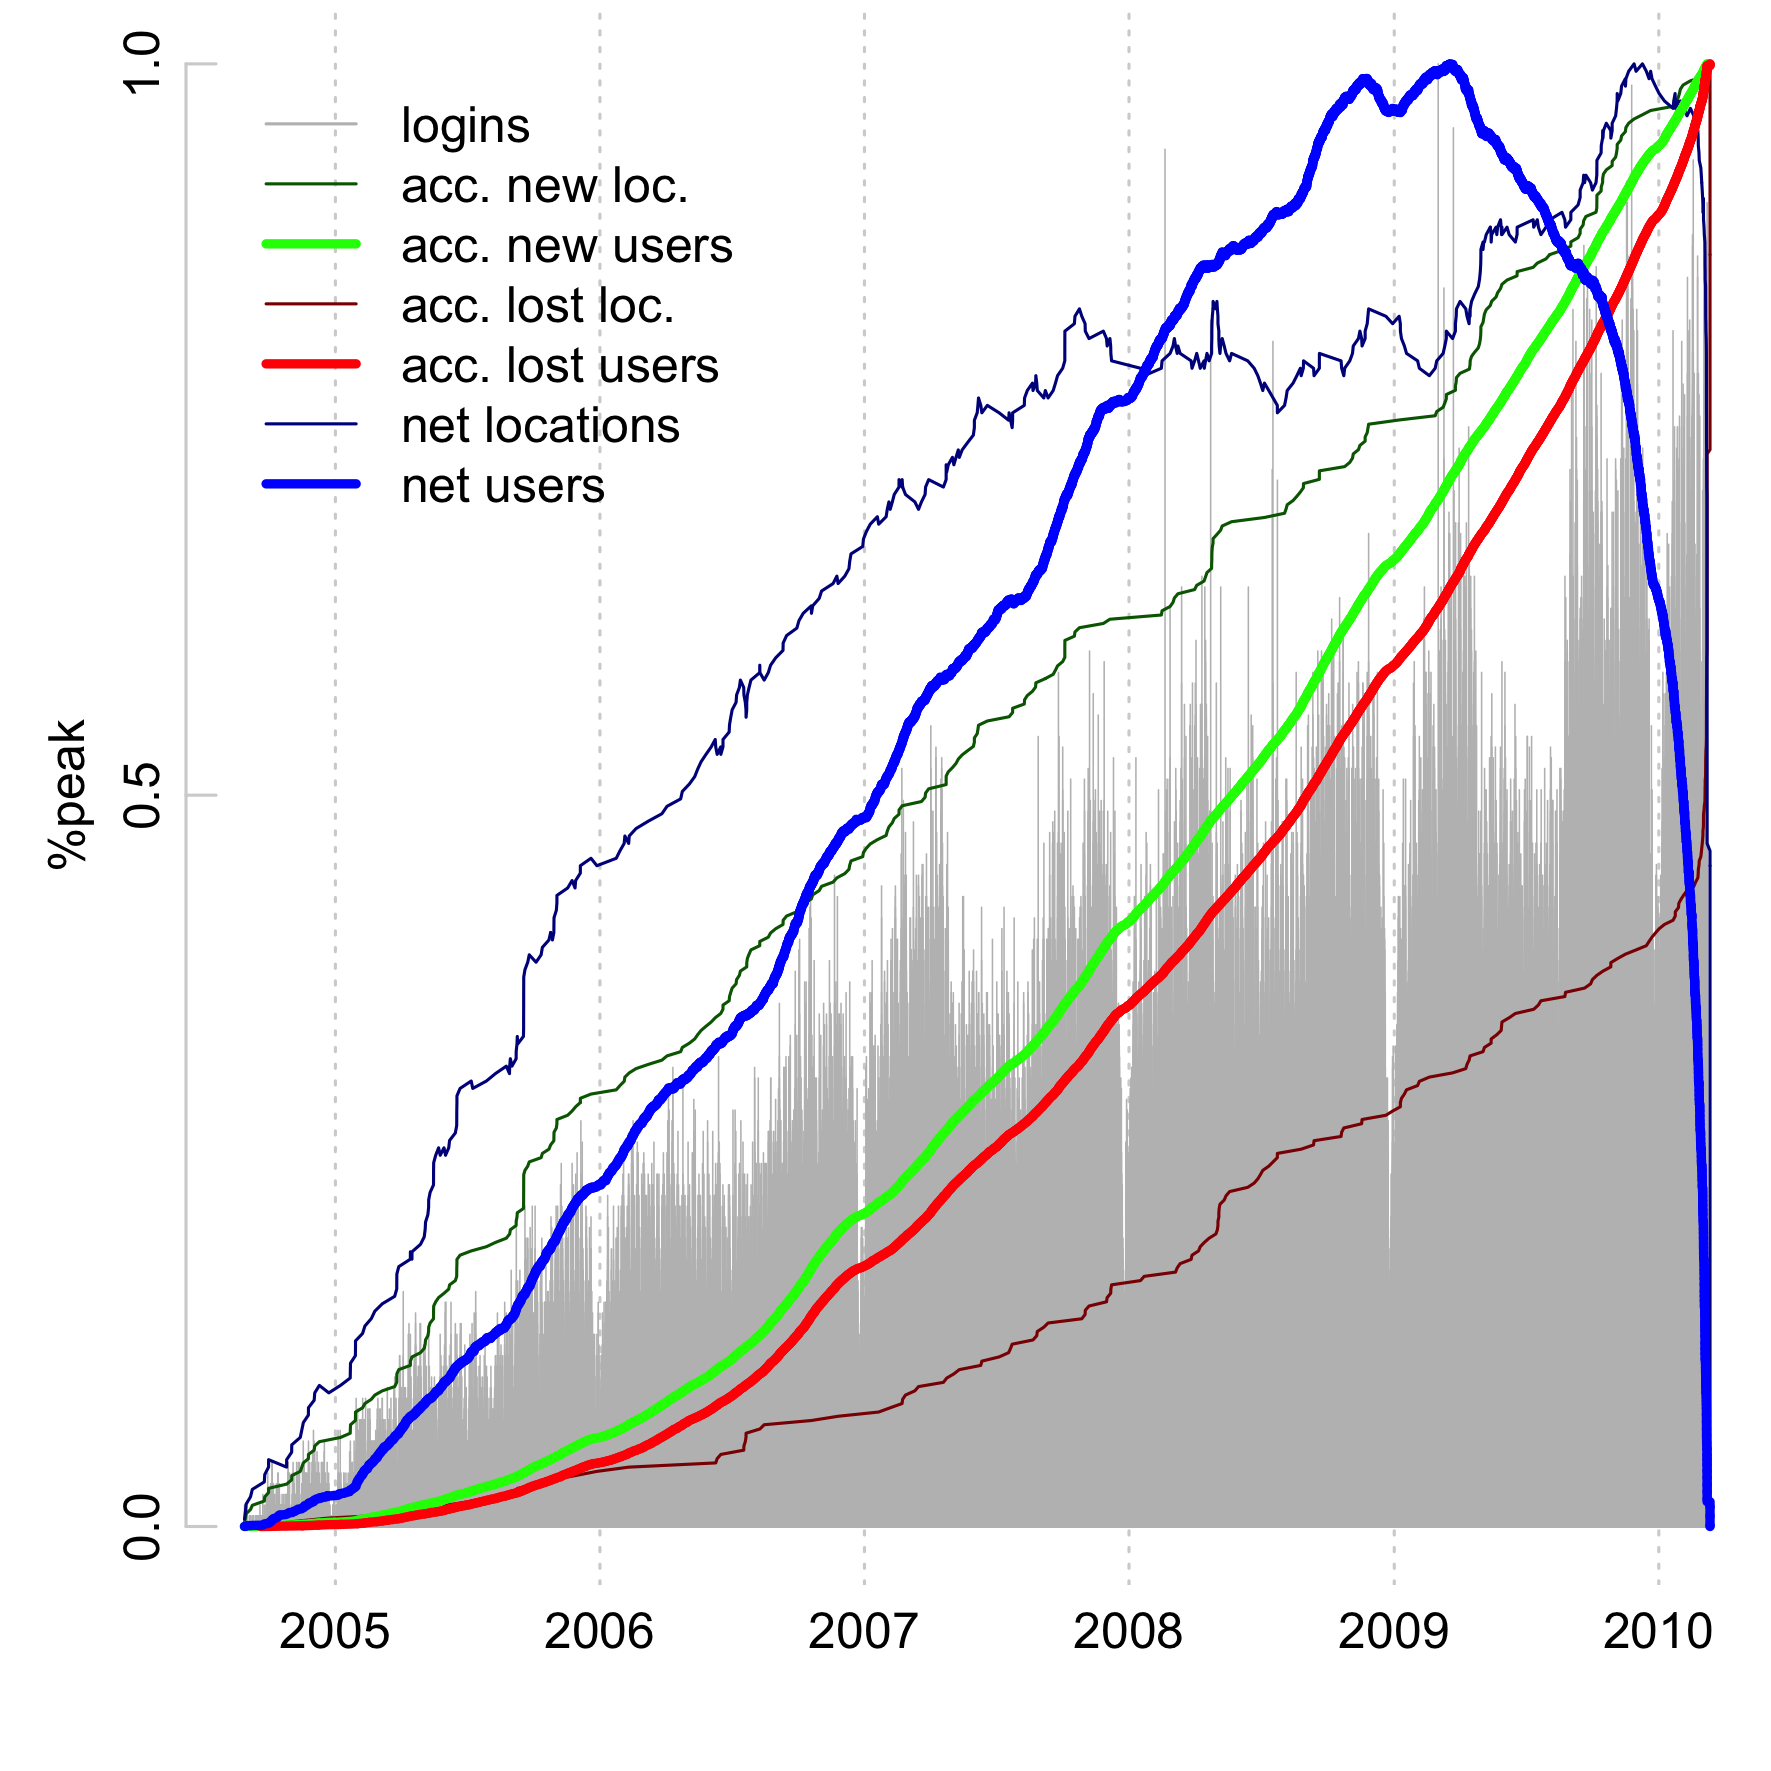
\includegraphics[width=1.0\linewidth]{dataReview.png}
      \end{figure}   
    \end{oneCol}
    %\spacer{}
    \begin{oneCol}
      \begin{figure}
        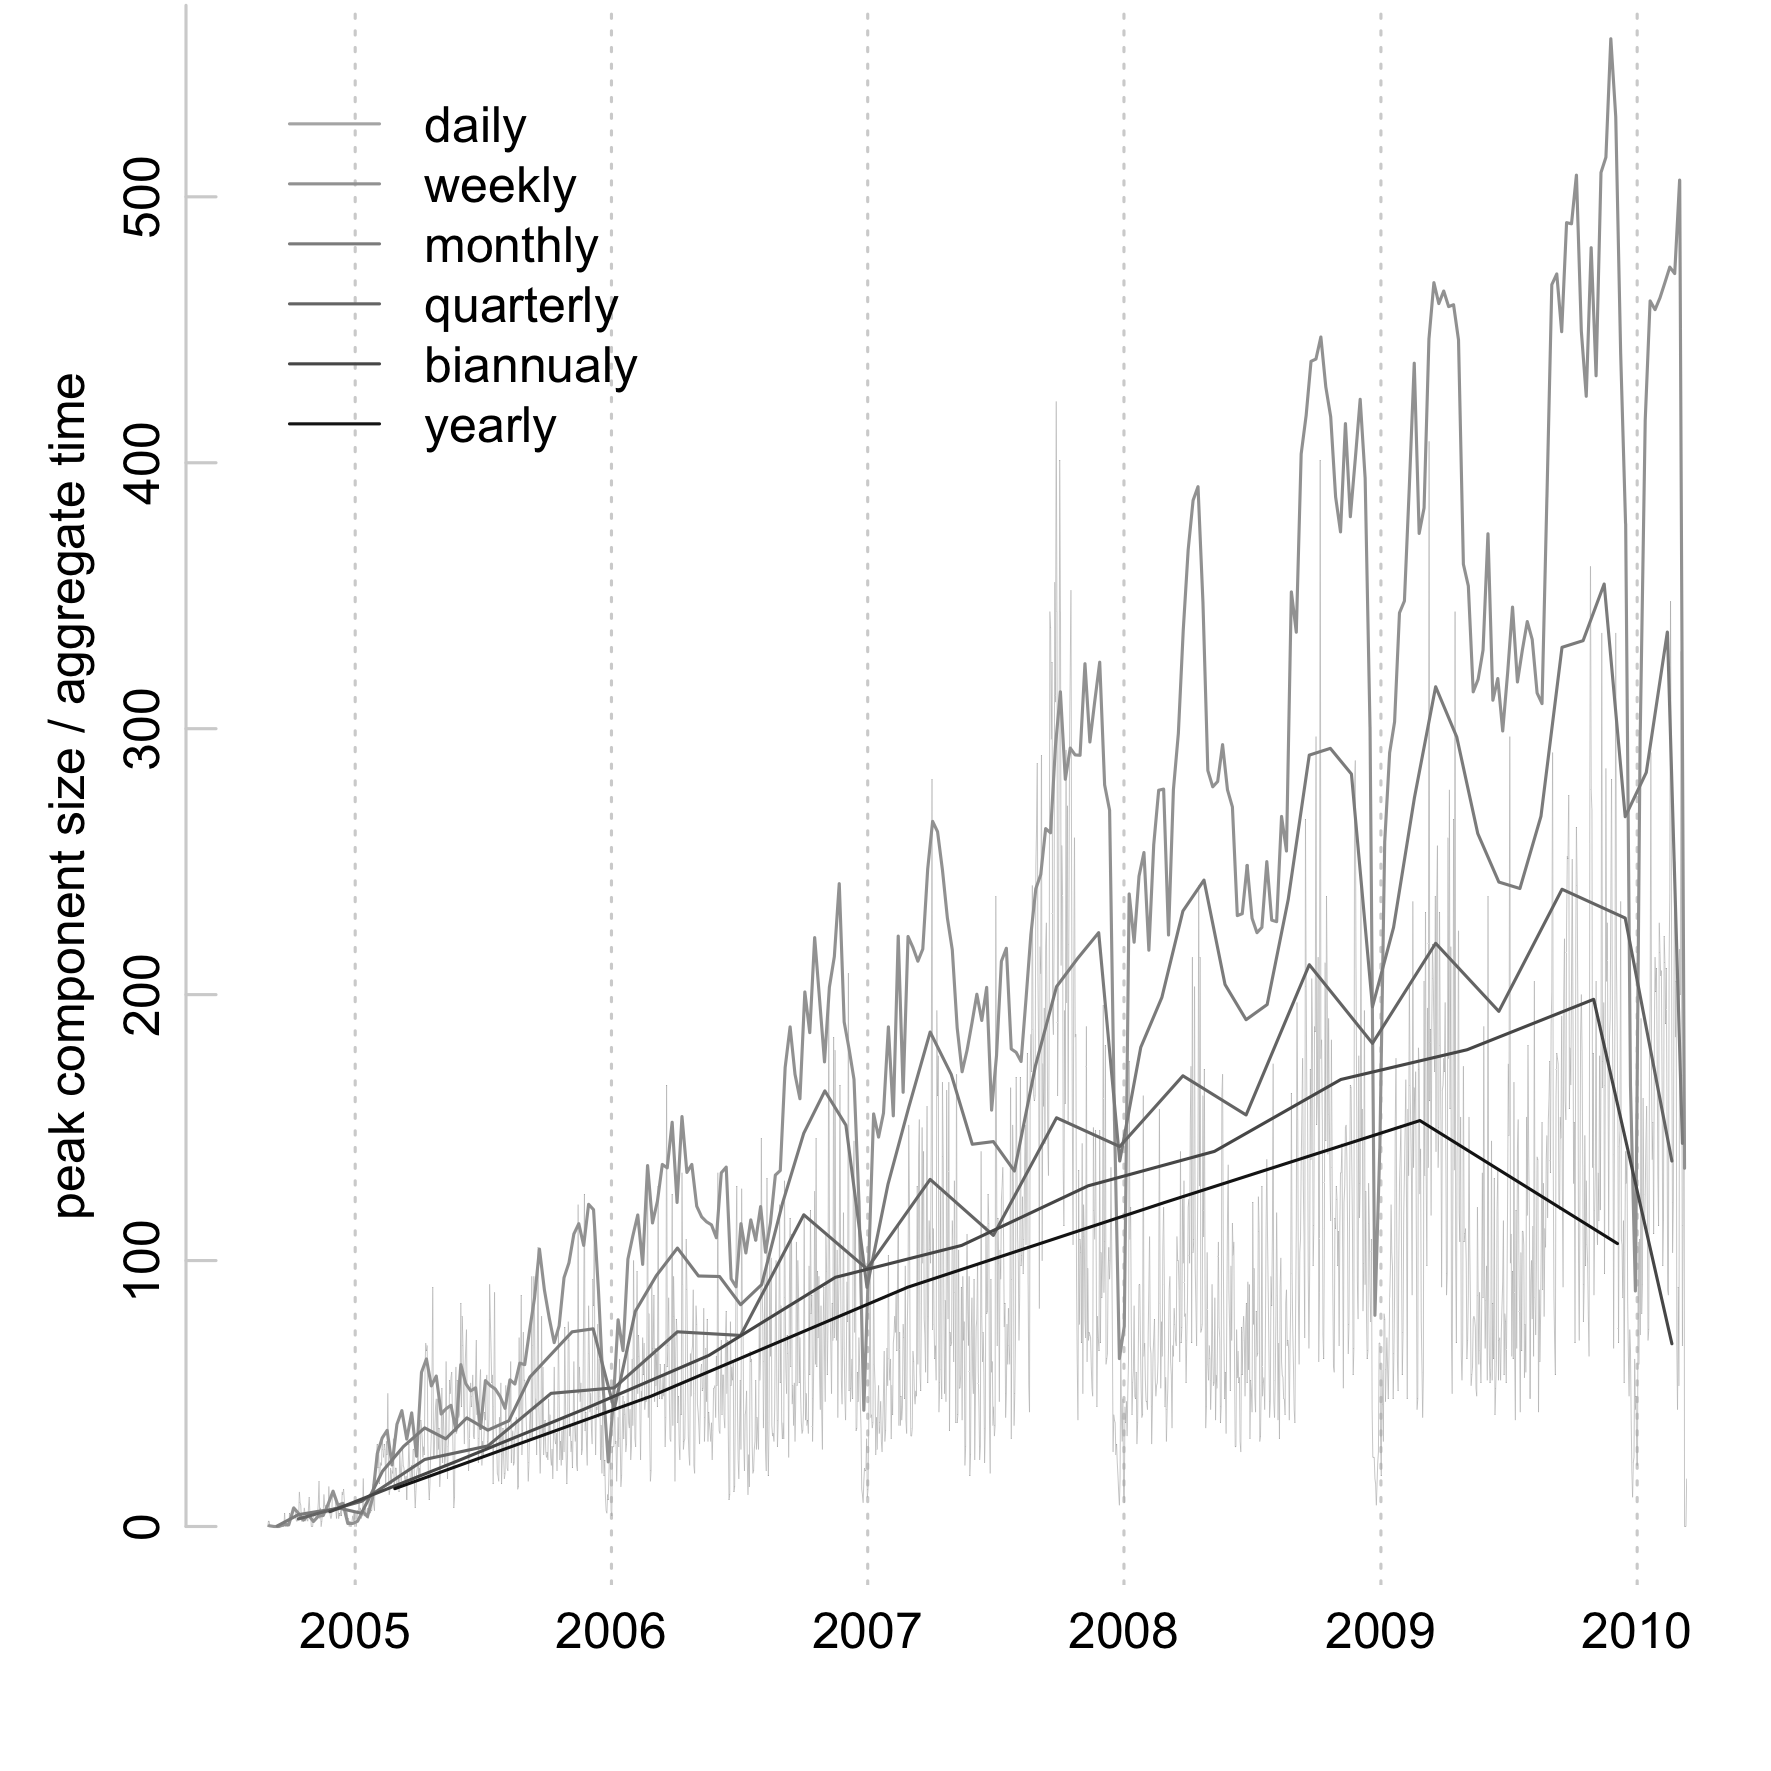
\includegraphics[width=1.0\linewidth]{maxComp.png}
      \end{figure}   
    \end{oneCol}
    %\spacer{}
    \begin{oneCol}
      \begin{figure}
        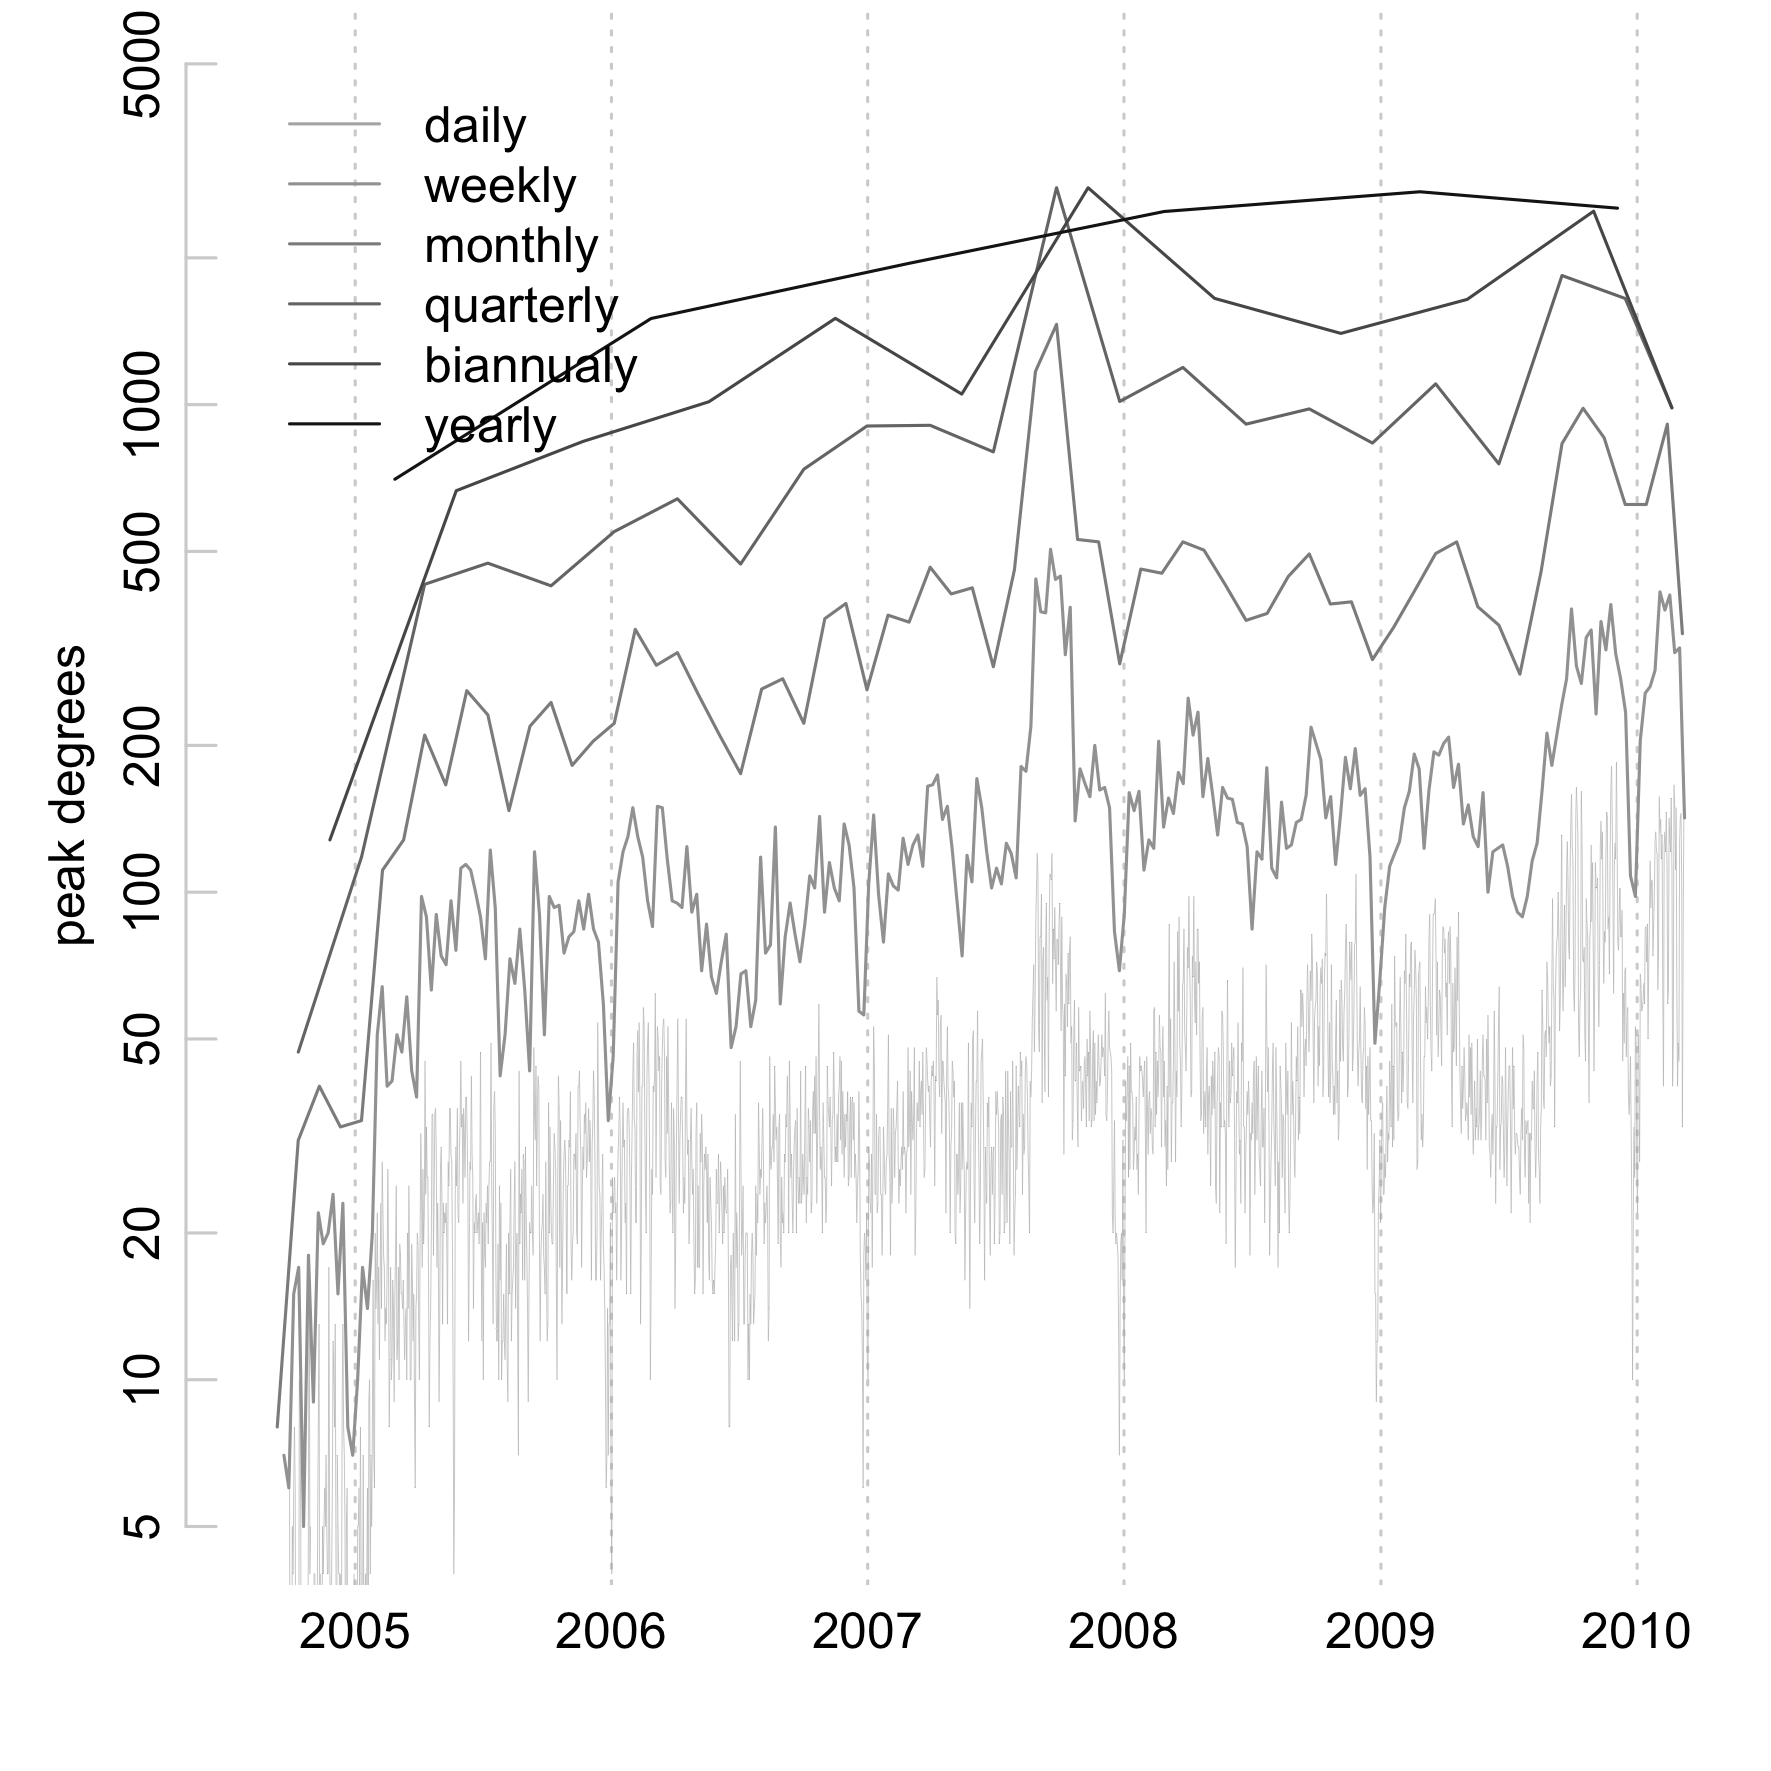
\includegraphics[width=1.0\linewidth]{maxEdges.png}
      \end{figure}   
    \end{oneCol}
    \end{columns}
    \end{block}
    
    \begin{block}{Results}
    \begin{columns}
    \begin{oneCol}
      \begin{figure}
        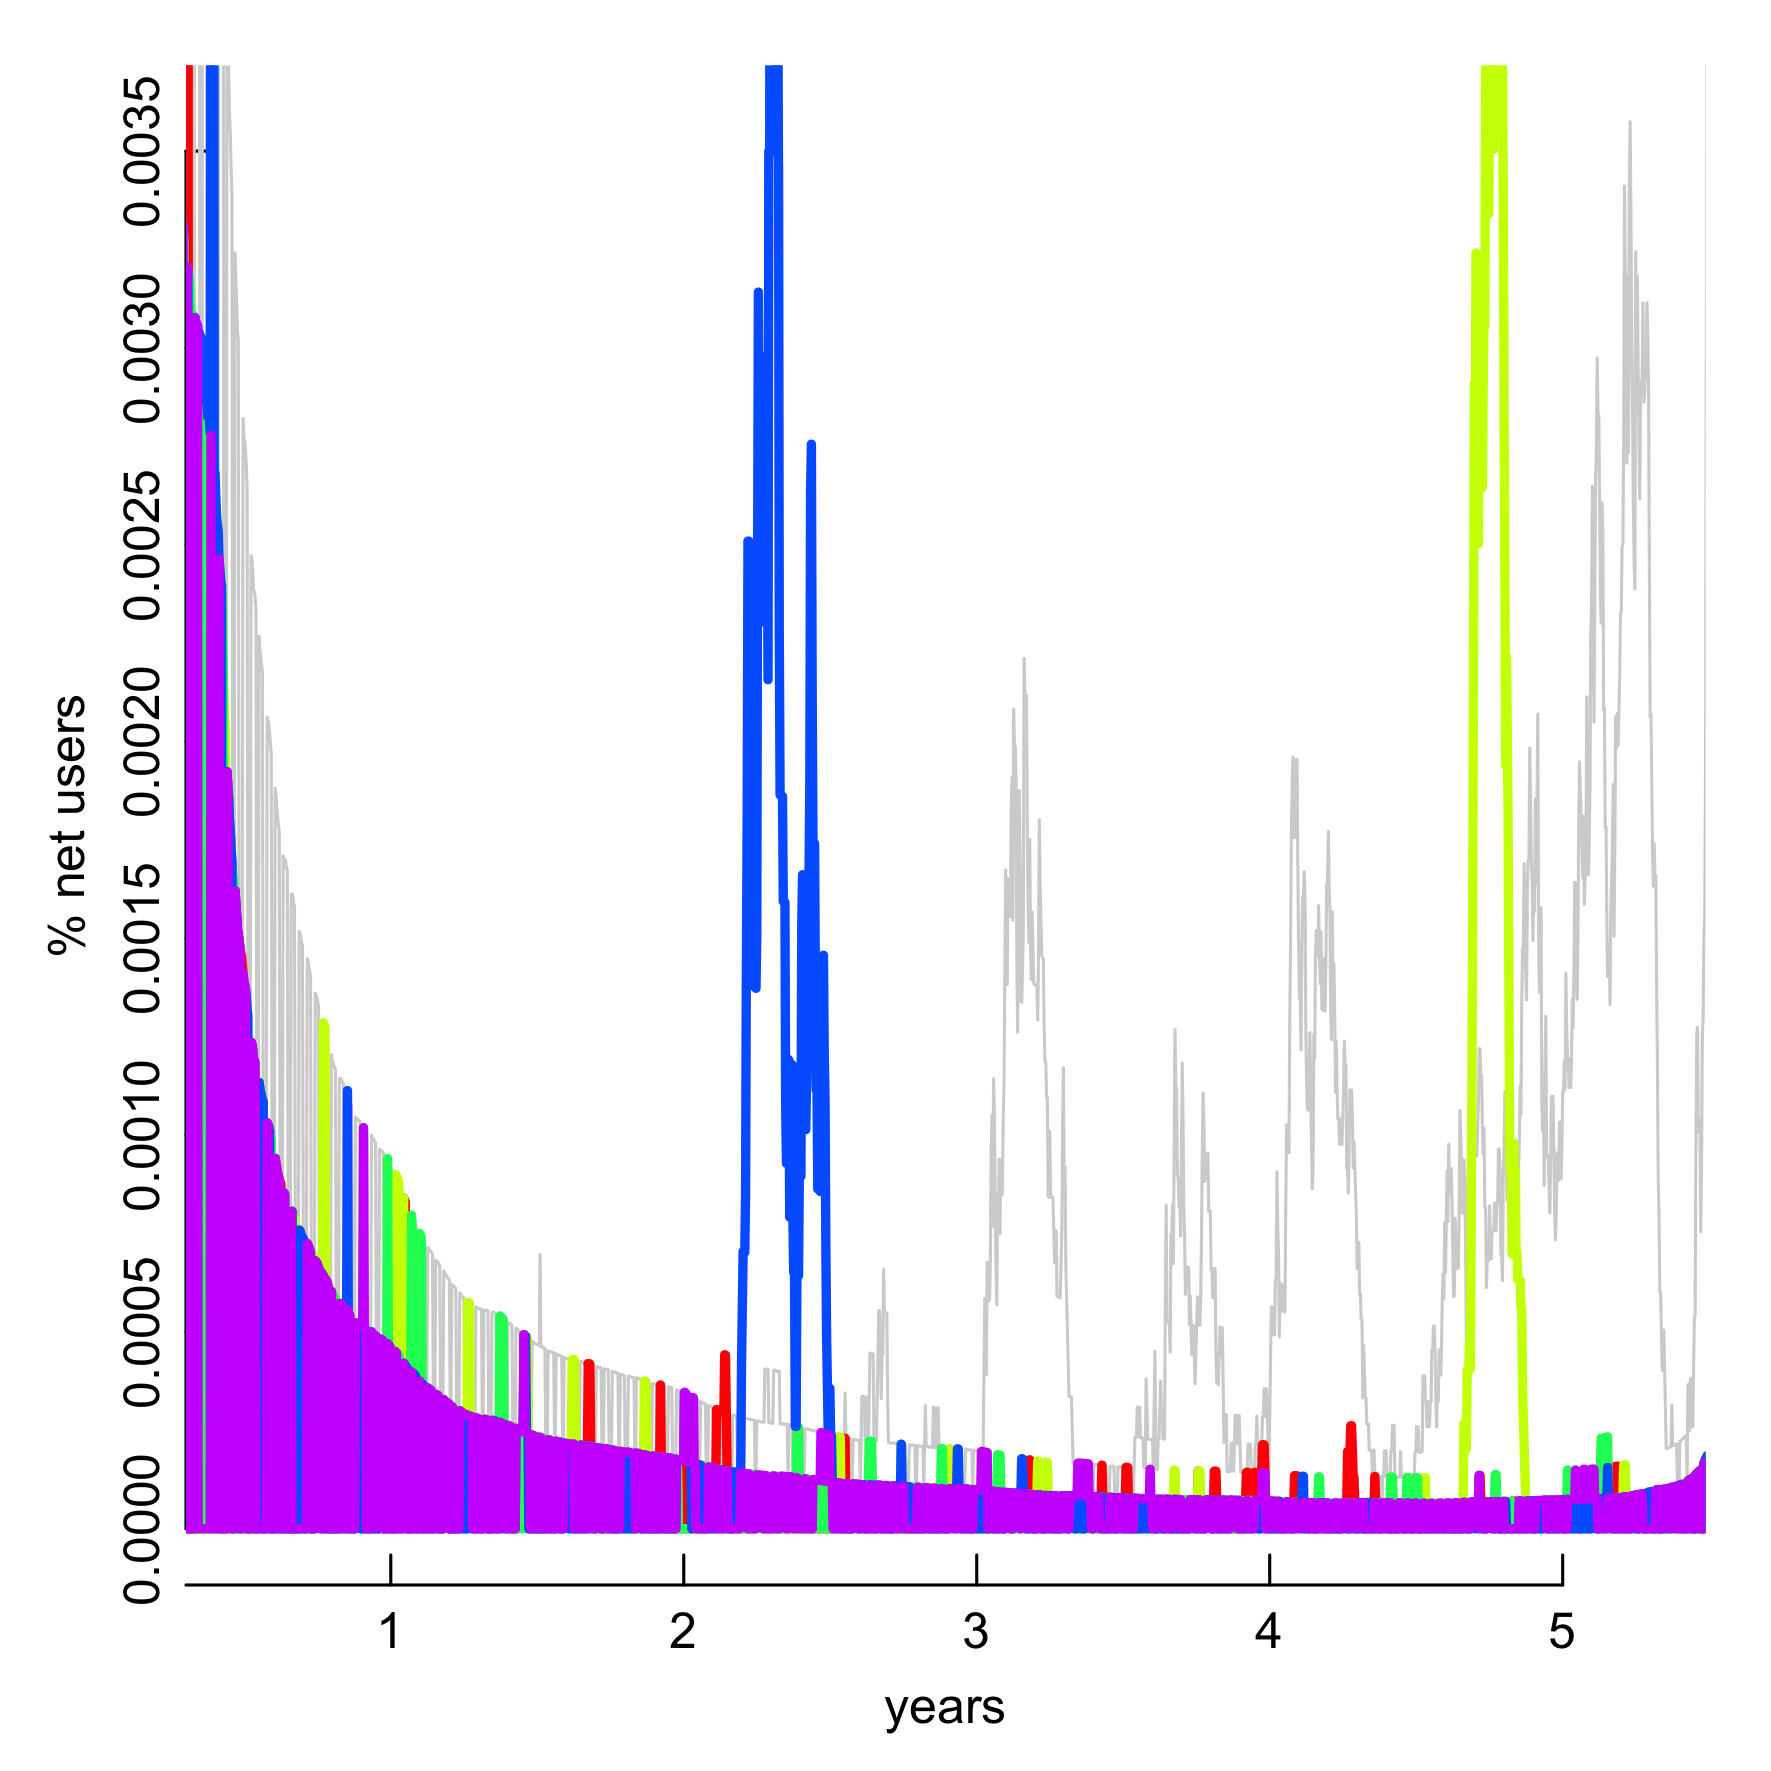
\includegraphics[width=1.0\linewidth]{out1.png}
      \end{figure}
      \begin{figure}
        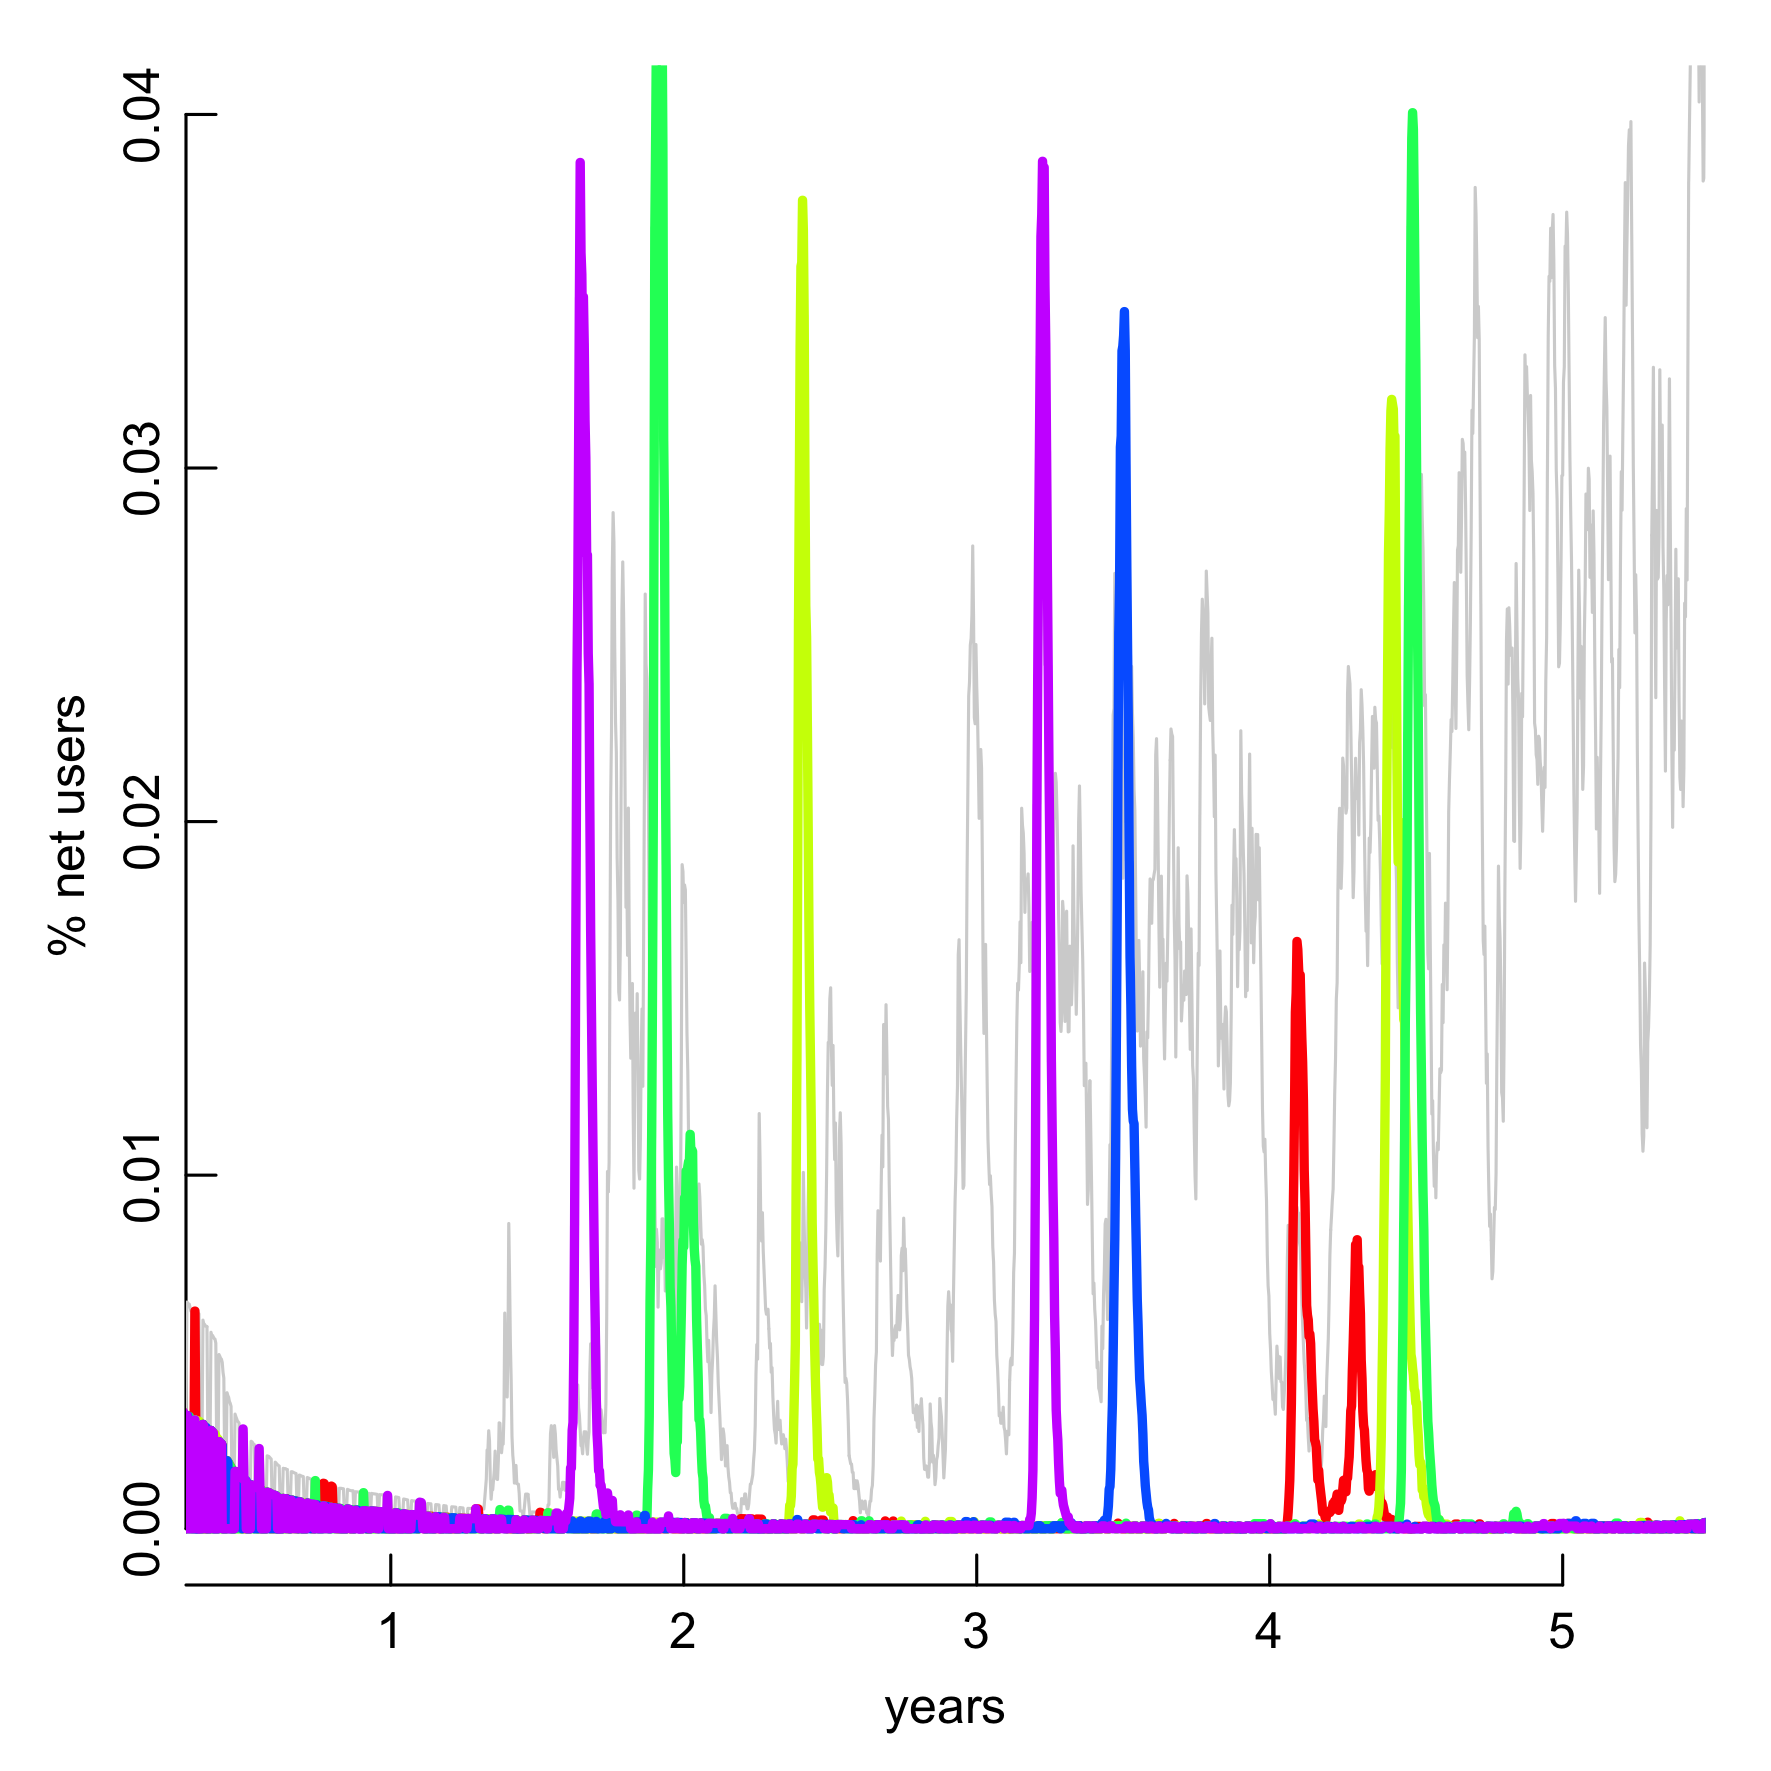
\includegraphics[width=1.0\linewidth]{out90.png}
      \end{figure}  
    \end{oneCol}
    %\spacer{}
    \begin{oneCol}
      \begin{figure}
        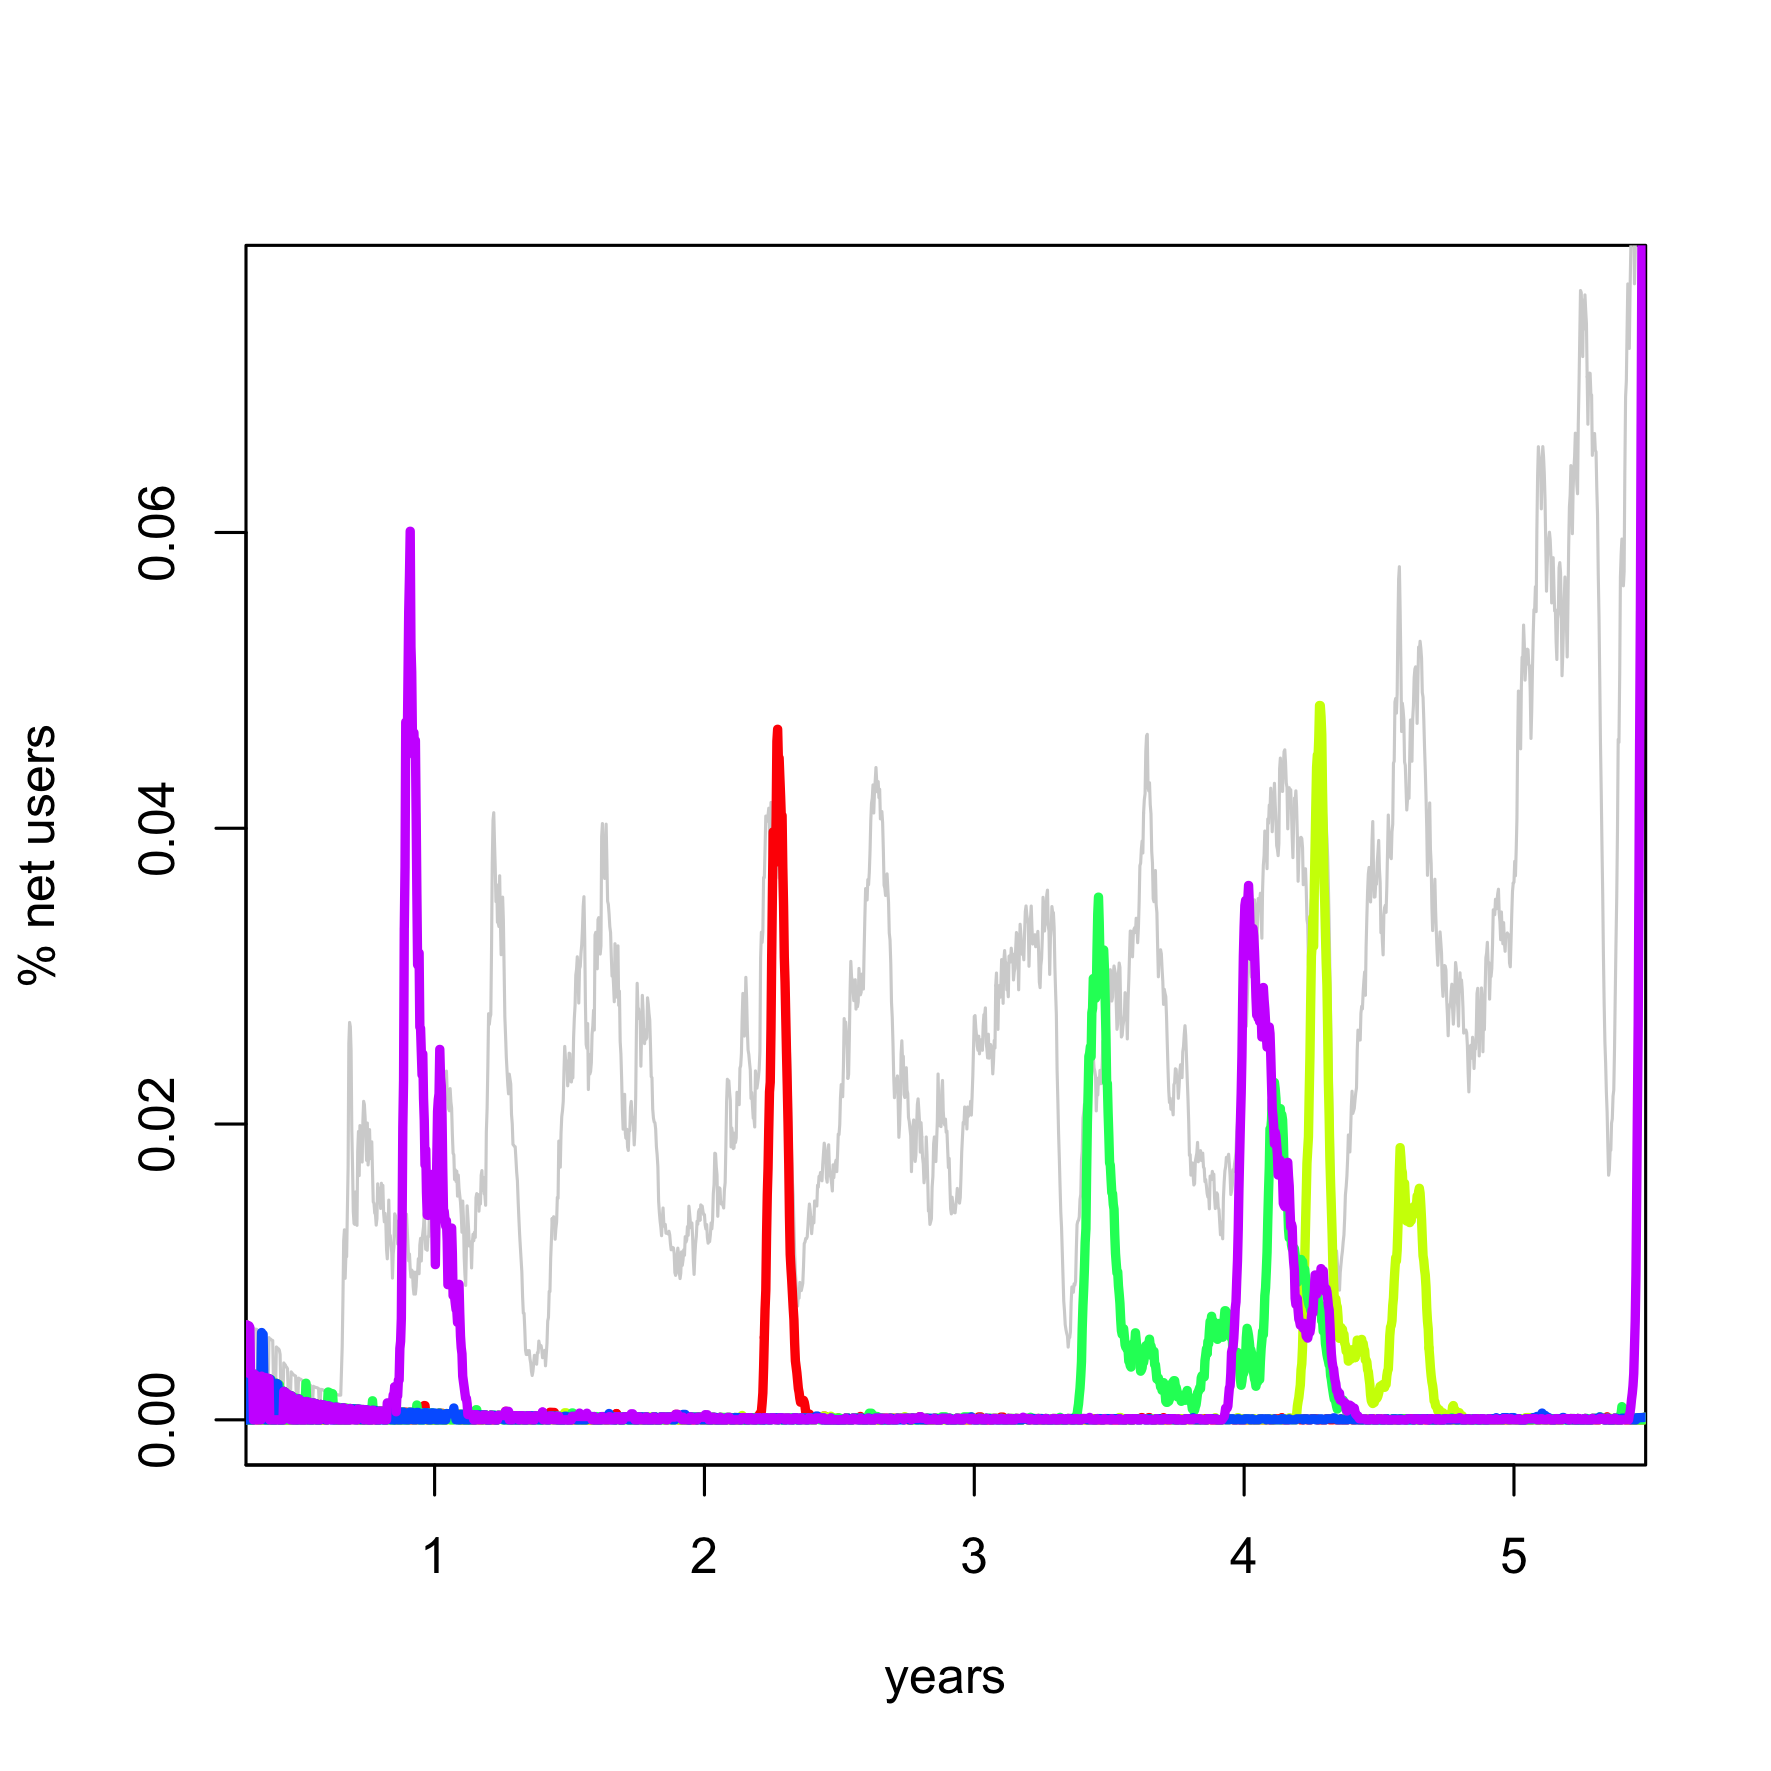
\includegraphics[width=1.0\linewidth]{out7.png}
      \end{figure}
      \begin{figure}
        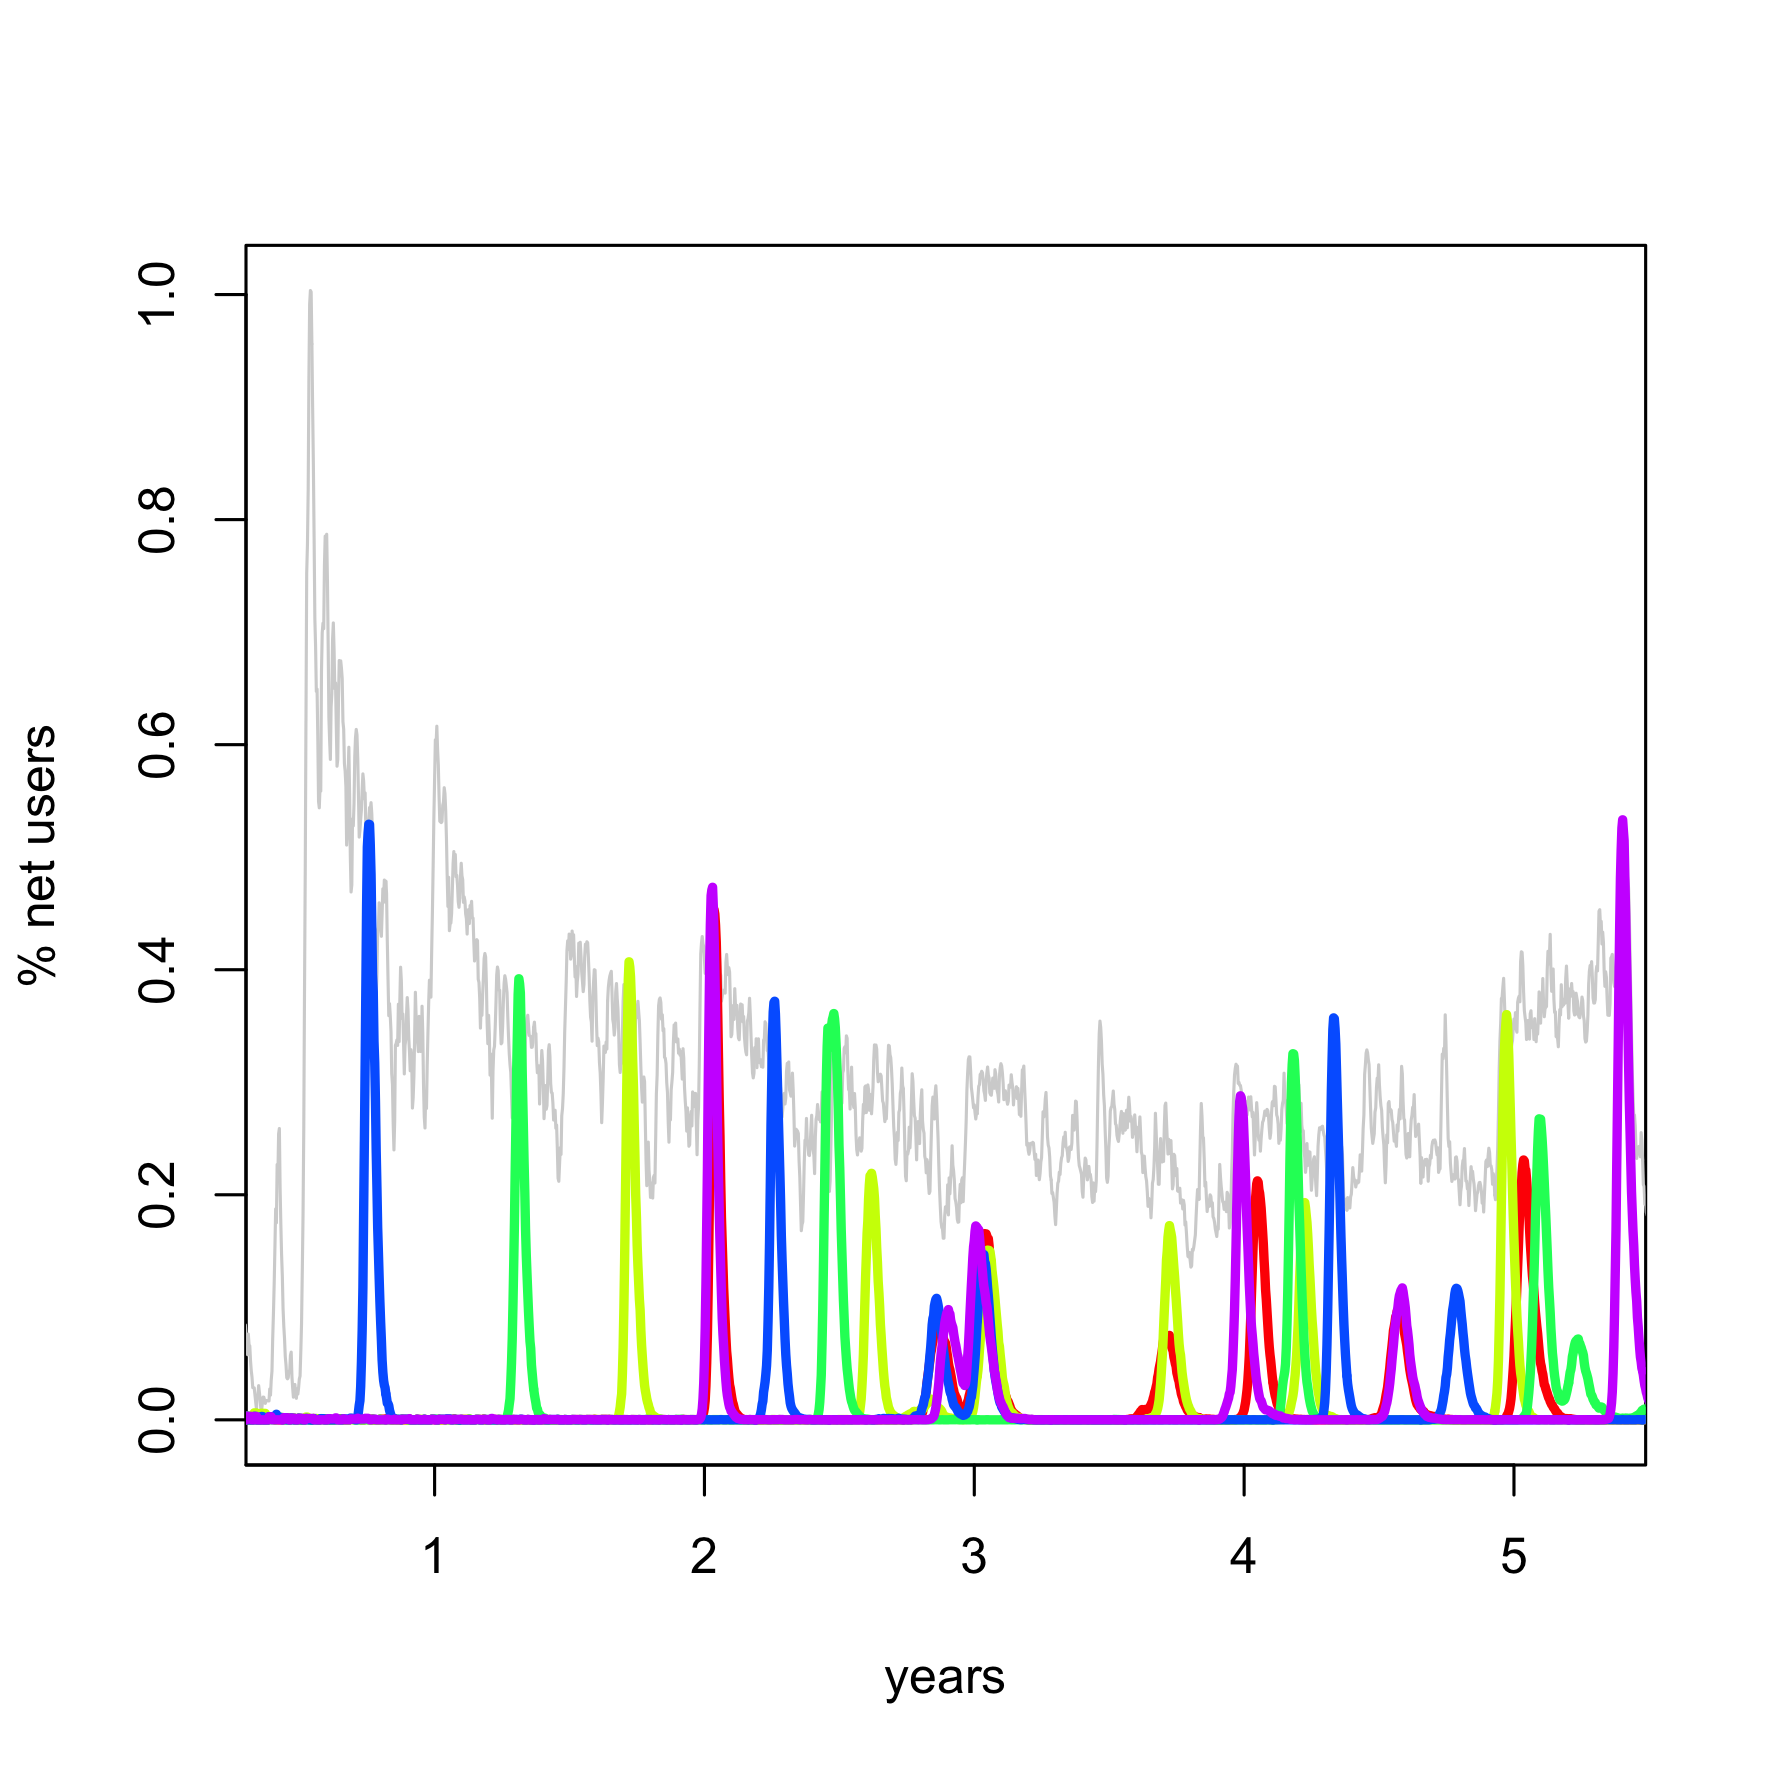
\includegraphics[width=1.0\linewidth]{out180.png}
      \end{figure}  
    \end{oneCol}
    %\spacer{}
    \begin{oneCol}
      \begin{figure}
        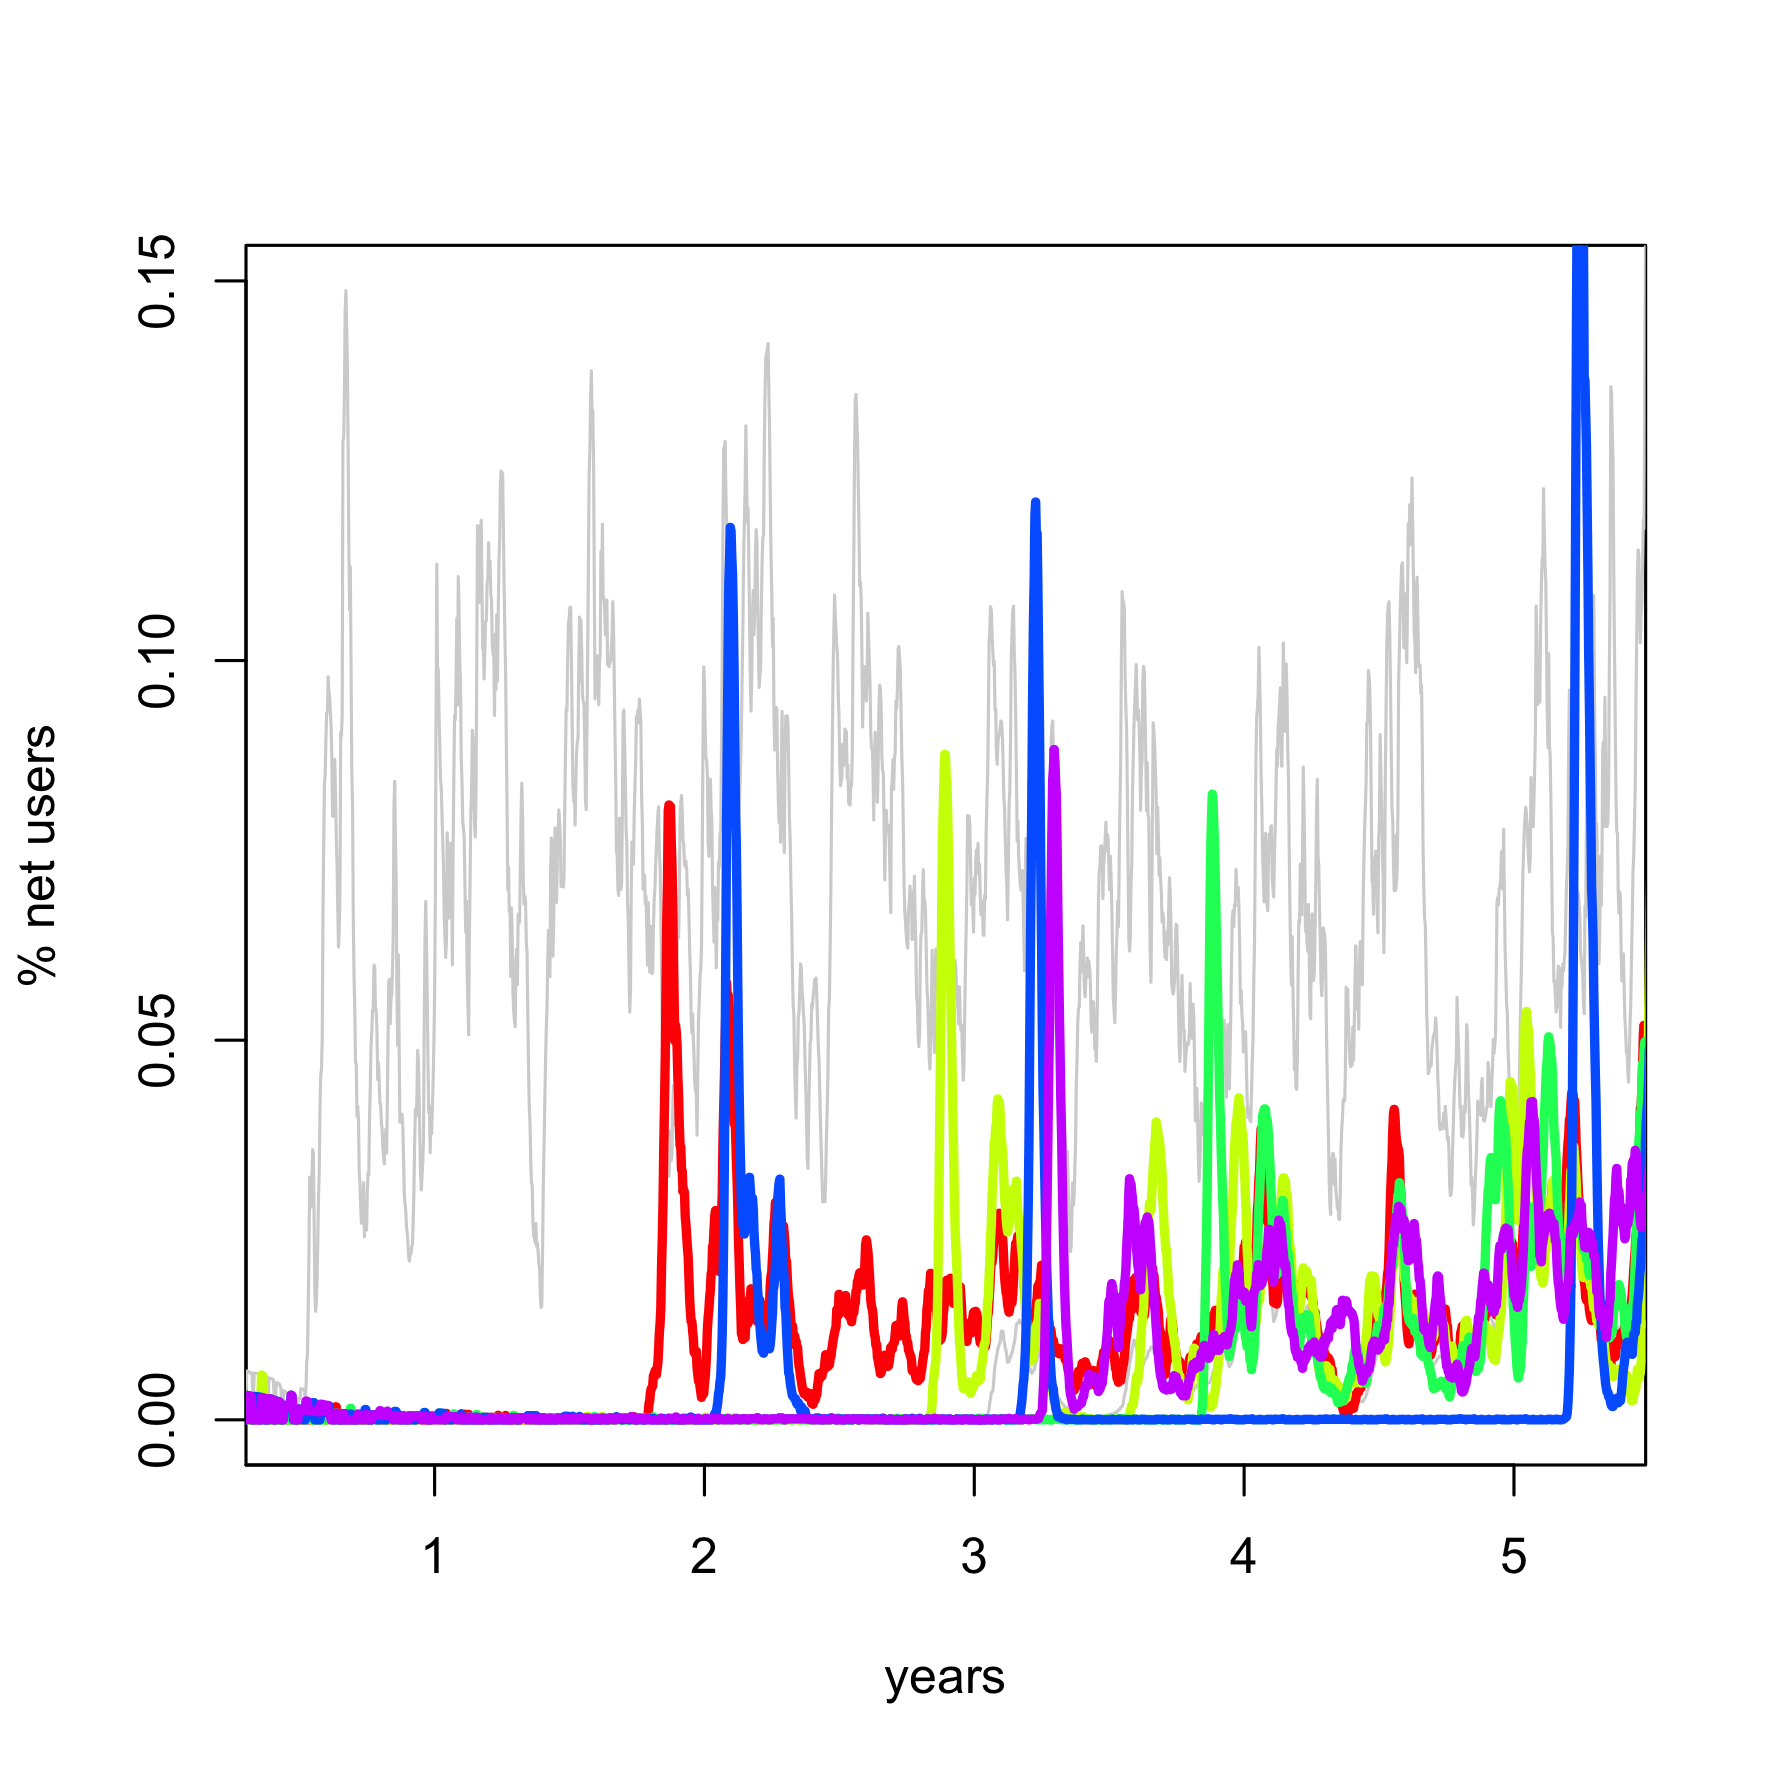
\includegraphics[width=1.0\linewidth]{out30.png}
      \end{figure}  
      \begin{figure}
        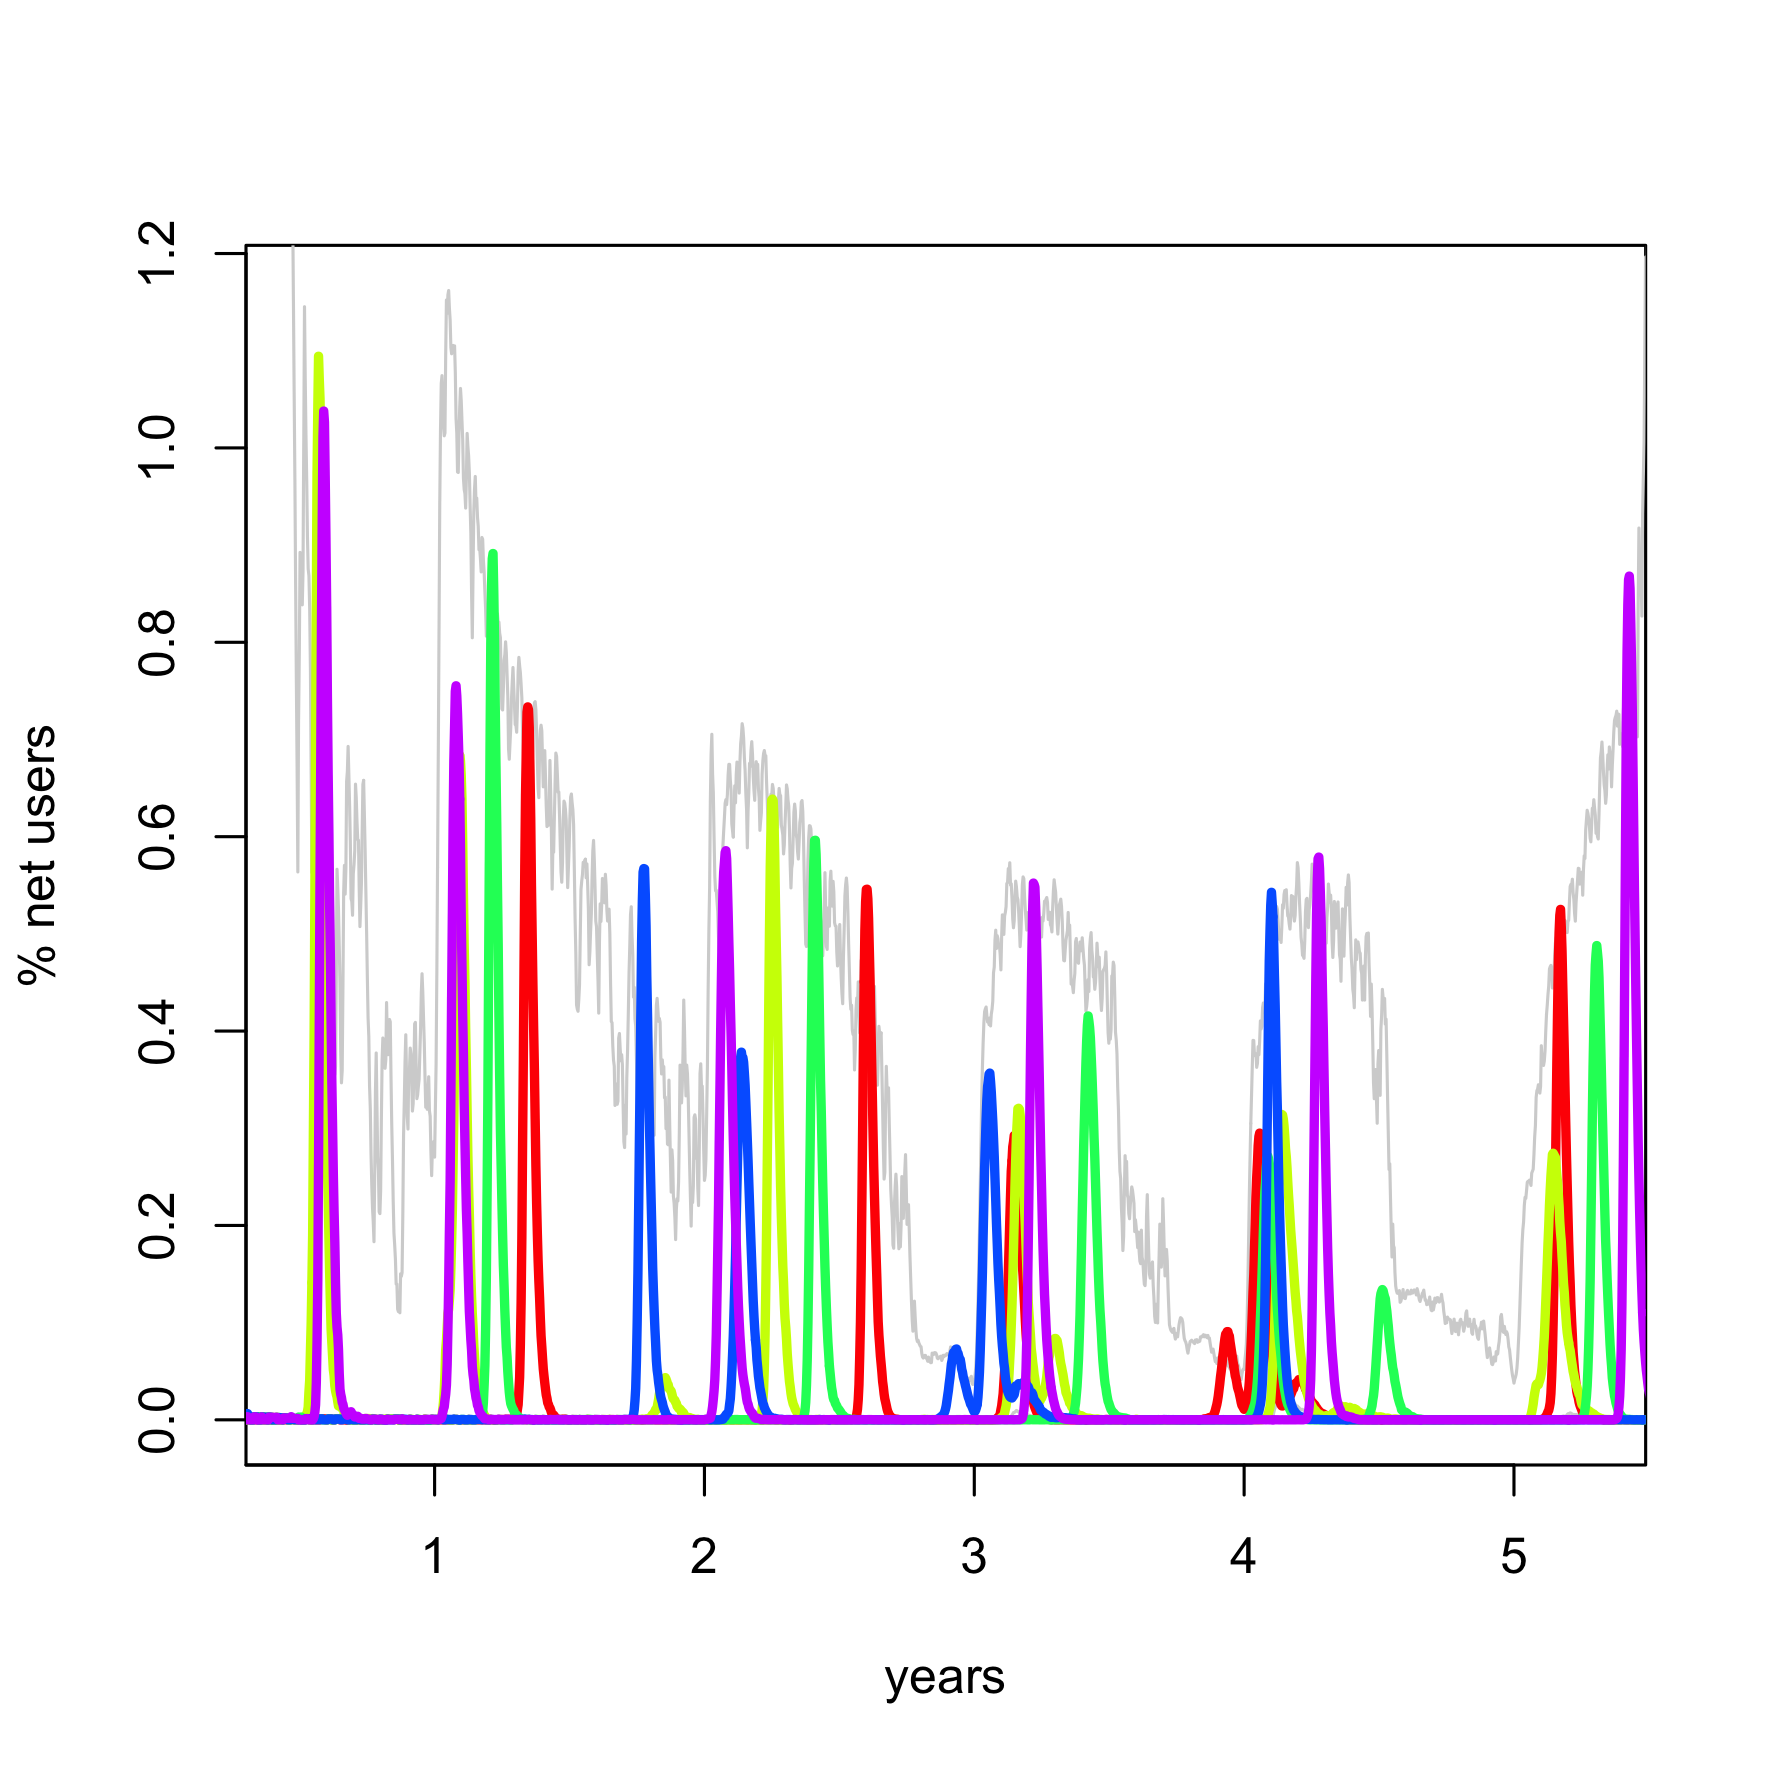
\includegraphics[width=1.0\linewidth]{out365.png}
      \end{figure}  
    \end{oneCol}
    \end{columns}
    
%    \begin{figure}
%<<plotfig1,fig=TRUE,echo=FALSE>>=
% graph.measure.plotting()
%@
%    
\includegraphics[width=0.8\linewidth]{placeholder.jpg}
%    \caption{The first figure should be a series of comparisons of network measures (e.g., degree distribution) for the totally aggregated network vs averaged values of the network aggregated at different time periods - 1 year, 1 month, 1 week, 1 day.  May also want to do some heat charts of those measures through time, since the averages might hide neat insights like seasonality.  I also think we could use some plots of something approximating edge weights -- like the distribution of edge duration proportion (time edge exists as fraction of interval).}
 %   \end{figure}
    
    \end{block}
    
    \end{threeCol}
    \spacer{}
    \end{columns}
  \end{frame}
  \end{document}
 



% 
% 
% %----------------------------------------------------------------------------------------
% %	ADDITIONAL INFORMATION
% %----------------------------------------------------------------------------------------
% 
% \begin{block}{Additional Information}
% 
% Maecenas ultricies feugiat velit non mattis. Fusce tempus arcu id ligula varius dictum. 
% \begin{itemize}
% \item Curabitur pellentesque dignissim
% \item Eu facilisis est tempus quis
% \item Duis porta consequat lorem
% \end{itemize}
% 
% \end{block}
% 
% %----------------------------------------------------------------------------------------
% %	REFERENCES
% %----------------------------------------------------------------------------------------
% 
% \begin{block}{References}
% 
% \nocite{*} % Insert publications even if they are not cited in the poster
% \small{\bibliographystyle{unsrt}
% \bibliography{sample}\vspace{0.75in}}
% 
% \end{block}
% 
% %----------------------------------------------------------------------------------------
% %	ACKNOWLEDGEMENTS
% %----------------------------------------------------------------------------------------
% 
% \setbeamercolor{block title}{fg=red,bg=white} % Change the block title color
% 
% \begin{block}{Acknowledgements}
% 
% \small{\rmfamily{Thank the data source + ARO grant that's paying for CABP to attend.}} \\
% 
% \end{block}
% 
% %----------------------------------------------------------------------------------------
% %	CONTACT INFORMATION
% %----------------------------------------------------------------------------------------
% 
% \setbeamercolor{block alerted title}{fg=black,bg=norange} % Change the alert block title colors
% \setbeamercolor{block alerted body}{fg=black,bg=white} % Change the alert block body colors
% 
% \begin{alertblock}{Contact Information}
% 
% \begin{itemize}
% \item Web: \href{http://github.com/pearsonca/epidemics-4talk}{http://github.com/pearsonca/epidemics-4talk}
% \item Email: \href{mailto:cap10@ufl.edu}{cap10@ufl.edu}, \href{mailto:thladish@ufl.edu}{thladish@ufl.edu}
% \end{itemize}
% 
% \end{alertblock}
% 
% \begin{center}
% \begin{tabular}{ccc}
% 
\includegraphics[width=0.4\linewidth]{logo.png} & \hfill & 
\includegraphics[width=0.4\linewidth]{logo.png}
% \end{tabular}
% \end{center}
% 
% %----------------------------------------------------------------------------------------
% 
% \end{column} % End of the third column
% 
% \end{columns} % End of all the columns in the poster
% 
% \end{frame} % End of the enclosing frame
% 
% \end{document}
